%%%%%%%%%%%%%%%%%%%%%%%%%%%%%%%%%%%%

\section{5.4. Calculando o poder para um teste de 2 amostras}

%%%%%%%%%%%%%%%%%%%%%%%%%%%%%%%%%%%%

\begin{frame}
\frametitle{}

\begin{center}
\begin{tabular}{l l | c c}
\multicolumn{2}{c}{} & \multicolumn{2}{c}{\textbf{Decisão}} \\
& & não rejeitar $H_0$ &  rejeitar $H_0$ \\
  \cline{2-4}
& $H_0$ verdade & \onslide<4->{\green{$1 - \alpha$}} & \onslide<2->{\orange{Erro tipo 1, $\alpha$}} \\
\raisebox{1.5ex}{\textbf{Verdade}} & $H_A$ verdade &  \onslide<3->{\orange{Erro tipo 2, $\beta$}} & \onslide<5->{\green{poder, $1 - \beta$}} \\
  \cline{2-4}
\end{tabular}
\end{center}

\pause

\begin{itemize}
\justifying
\item O erro tipo 1 acontece quando se rejeita $H_0$ quando ela é verdadeira, e a probabilidade de fazer isso é $\alpha$ (nível de significância).

\pause 
\justifying
\item O erro tipo 2 acontece quand se falha em rejeitar $H_0$ ela não é verdadeira, e a probabilidade de fazer isso é $\beta$ (um pouco mais complicado de calcular).

\pause 
\justifying
\item \hl{Poder} de um teste é a probabilidade de rejeitar corretamente $H_0$, e a probabilidade de fazer isso é $ 1 - \beta $.

\pause 
\justifying
\item Nos testes de hipóteses, queremos manter $\alpha$ e $\beta$ baixo, mas existem compensações inerentes.

\end{itemize}

\end{frame}

%%%%%%%%%%%%%%%%%%%%%%%%%%%%%%%%%%%%

\begin{frame}
\frametitle{Taxa de erro tipo 2}
\justifying
Se a hipótese alternativa é realmente verdadeira, qual é a chance de fazermos um Erro Tipo 2, ou seja, deixamos de rejeitar a hipótese nula mesmo quando deveríamos rejeitá-la?

\begin{itemize}
\justifying
\item A resposta não é obvia.
\justifying
\item Se a média real da população estiver muito próxima do valor da hipótese nula, será difícil detectar uma diferença (e rejeitar $ H_0 $).
\justifying
\item Se a média real da população for muito diferente do valor da hipótese nula, será mais fácil detectar uma diferença.
\justifying
\item Claramente, $\beta$ depende do \hl{tamanho do efeito} ($\delta$)
\end{itemize}

\end{frame}

%%%%%%%%%%%%%%%%%%%%%%%%%%%%%%%%%%%%

\begin{frame}
\frametitle{Exemplo - Pressão Arterial (PA), hipóteses}
\justifying
{\dq
{\footnotesize
Suponha que uma empresa farmacêutica tenha desenvolvido uma nova droga para baixar a pressão sanguínea e esteja preparando um ensaio clínico para testar a eficácia da droga. Eles recrutam pessoas que estão tomando uma medicação padrão de pressão sanguínea, e metade dos indivíduos recebe a nova droga (tratamento) e a outra metade continua a tomar a medicação atual com pílulas genéricas para garantir a cegueira (controle). Quais são as hipóteses para um teste de hipóteses bilateral neste contexto?
}
}

\pause

\soln{
\begin{align*}
H_0&: \mu_{tratamento} - \mu_{controle} = 0 \\
H_A&: \mu_{tratamento} - \mu_{controle} \ne 0  
\end{align*}
}

\end{frame}

%%%%%%%%%%%%%%%%%%%%%%%%%%%%%%%%%%%%

\begin{frame}
\frametitle{Exemplo - BP, erro padrão}
\justifying
{\dq
{\footnotesize
Suponha que os pesquisadores gostariam de executar o ensaio clínico em pacientes com pressão arterial sistólica entre 140 e 180 mmHg. Suponha que estudos publicados anteriormente sugiram que o desvio padrão das pressões sanguíneas dos pacientes é de cerca de 12 mmHg e a distribuição das pressões sanguíneas dos pacientes será aproximadamente simétrica. Se tivéssemos 100 pacientes por grupo, qual seria o erro padrão aproximado para diferença nas médias amostrais dos grupos de tratamento e controle?
}
}

\pause

\soln{
\[ SE = \sqrt{ \frac{12^2}{100} + \frac{12^2}{100} } = 1.70 \]
}

\end{frame}

%%%%%%%%%%%%%%%%%%%%%%%%%%%%%%%%%%%%

\begin{frame}
\frametitle{Exemplo - BP, tamanho de efeito mínimo necessário para rejeitar $H_0$}
\justifying
{\dq
{\footnotesize
Para que valores da diferença entre as médias observadas da pressão arterial nos grupos tratamento e controle (tamanho do efeito) rejeitaríamos a hipótese nula no nível de significância de 5\%?}
}

\pause

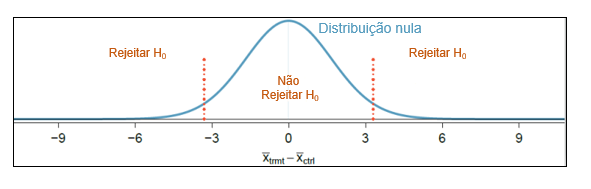
\includegraphics[width=\textwidth]{5-4_power/power_null_B_0_1-7_with_rejection_region.png}

\pause
\small{
\justifying
A diferença deve ser pelo menos 
\[ 1.96 * 1.70 = 3.332 \] 
\justifying
ou no máximo 
\[ -1.96 * 1.70 = 3.332. \]
}
\end{frame}

%%%%%%%%%%%%%%%%%%%%%%%%%%%%%%%%%%%%

\begin{frame}
\frametitle{Exemplo - BP, poder}
\justifying
{\dq
{\footnotesize
Suponha que os pesquisadores da empresa se preocupem em encontrar qualquer efeito na pressão arterial que seja de 3 mmHg ou maior em relação à medicação padrão. Qual é o poder do teste que pode detectar esse efeito?
}}

\pause

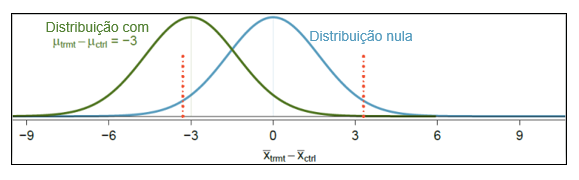
\includegraphics[width=\textwidth]{5-4_power/power_null_C_0_1-7_with_alt_at_3.png}

\pause

\[ Z = \frac{-3.332 - (-3)}{1.70} = -0.20 \]

\pause

\[ P(Z < -0.20) = 0.4207 \]

\end{frame}

%%%%%%%%%%%%%%%%%%%%%%%%%%%%%%%%%%%%

\begin{frame}
\frametitle{Exemplo - BP, tamanho de amostra necessário para 80\% de poder}
\justifying
{\dq
{\footnotesize
Qual tamanho de amostra levará a uma poder de 80\% para este teste?
}}

\pause

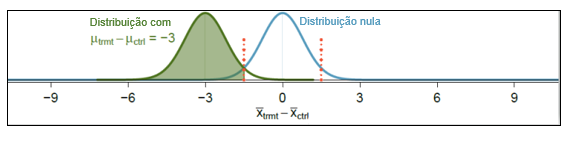
\includegraphics[width=\textwidth]{5-4_power/power_null_0_0-76_with_alt_at_3_and_shaded.png}

\pause
\small{
\[ SE = \frac{3}{2.8} = 1.07142 \]

\pause

\[ 1.07142 = \sqrt{ \frac{12^2}{n} + \frac{12^2}{n} } \]

\pause

\[ n = 250.88 \rightarrow n \ge 251 \]
}
\end{frame}

%%%%%%%%%%%%%%%%%%%%%%%%%%%%%%%%%%%%

\begin{frame}
\frametitle{Recapitulando}

\begin{itemize}
\justifying
\item Calcule o tamanho de amostra necessário para um nível desejado de poder.
\justifying
\item Calcule a poder para uma faixa de tamanhos de amostra e, em seguida, escolha o tamanho da amostra que produz a poder desejado (geralmente 80\% ou 90\%).
\end{itemize}
\begin{center}
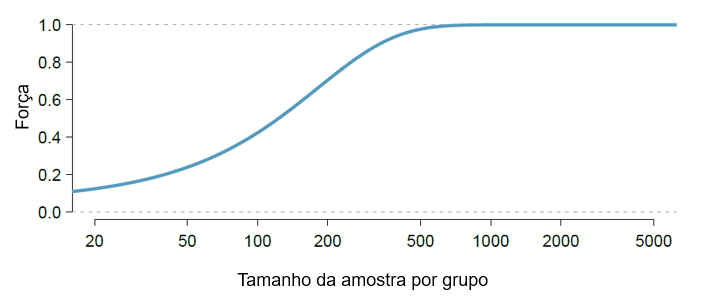
\includegraphics[width=0.7\textwidth]{5-4_power/power_curve_neg-3.png}
\end{center}

\end{frame}

%%%%%%%%%%%%%%%%%%%%%%%%%%%%%%%%%%%%

\begin{frame}
\frametitle{Alcançar o poder desejado}
\justifying
Existem várias maneiras de aumentar o poder (e, portanto, diminuir a taxa de erro do tipo 2):

\pause

\begin{enumerate}
\justifying
\item Aumentar o tamanho da amostra

\pause
\justifying
\item Diminuir o desvio padrão da amostra, que essencialmente tem o mesmo efeito que aumentar o tamanho da amostra (diminuirá o erro padrão). Com um $s$ menor, temos uma chance maior de distinguir o valor nulo da estimativa pontual observada. Isso é difícil de assegurar, mas um processo de medição cauteloso e a limitação da população para que ela seja mais homogênea podem ajudar.

\end{enumerate}
\end{frame}
%%%%%%%%%%%%%%%%%%%%%%%%%%%%%%%%%%%%

\begin{frame}
\frametitle{Alcançar o poder desejado}

\begin{enumerate}[3.]

\justifying
\item Aumente $\alpha$, o que aumentará a probabilidade de rejeitar $H_0$ (mas observe que isso tem o efeito colateral de aumentar a taxa de erro de tipo 1).

\end{enumerate}


\pause
\begin{enumerate}[4.]
\justifying
\item Considere um tamanho de efeito maior. Se a verdadeira média da população estiver na hipótese alternativa, mas próxima do valor nulo, será mais difícil detectar uma diferença.

\end{enumerate}


\end{frame}

%%%%%%%%%%%%%%%%%%%%%%%%%%%%%%%%%%%%

